\clearpage

\subsection{Register Write Interface} \label{chap:registerwrite}
The ASIC contains a set of registers to enable internal DACs, which have different purposes such as fine tune of current charge, enable/disable Test Pattern Register, and so on. These register can only be accessed through the register interface pins, see table \ref{tab:regwrite}. This type of communication is a 19-Bit wide word followed by a signal transaction between SIN and PCLK, see figure \ref{fig:TC_writeregister}. The SIN signal must be shifted out on each rising edge of the SCLK clock, the ASIC samples the SIN input on the falling edge.

\subsubsection*{Pinout(s)}
\begin{table}[H]
\centering
\begin{tabu}{| c | p{0.15\linewidth} | p{0.2\linewidth} | p{0.4\linewidth} |}
\hline
\HEADTABLE
Pin\# & Pin Name & Pin Type & Description\\
\hline
35  & SIN   & Digital Input & Serial Input data\\
36	& SCLK	& Digital Input	& Serial clock advance \\
37	& PCLK	& Digital Input	& Parallel clock load	\\
38	& SHout	& Digital Output & Serial Shift Out\\
\hline
\end{tabu}
\caption{\label{tab:regwrite} Register interface Pins}
\end{table}


\subsubsection*{Requirement(s)}
\begin{table}[H]
\centering
\begin{tabu}{   | p{0.1\linewidth} | p{0.8\linewidth} |}
\hline
\HEADTABLE
Req\# & Description\\
\hline
1	& PCLK Pulse shall be at least 100 ns wide\\
2	& SIN shall start before PCLK last pulse\\
3	& MSB First\\
4 & ASIC samples on falling edge, data is shifted out on the rising edge\\
\hline
\end{tabu}
\caption{\label{tab:reqregwrite} Requirement for the register write interface}
\end{table}


\subsubsection*{Payload}
\begin{table}[H]
\centering
\begin{tabu}{  | p{0.1\linewidth} | p{0.8\linewidth} |}
\hline
\HEADTABLE
Bits & Description\\
\hline
18 - 12	& Register Address \\
11 - 0	& 12-Bit Data  	\\
\hline
\end{tabu}
\caption{\label{tab:reg76} TARGETC 19-Bit Register payload}
\end{table}

\subsubsection*{Interface sequence}
\begin{figure}[H]
\centering
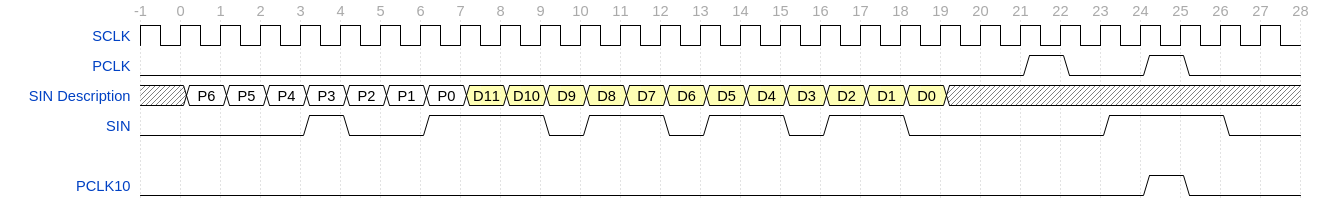
\includegraphics[width=1\textwidth]{figures/wavedrom/registers2.png}\\
\caption{\label{fig:TC_writeregister} Register Write Sequence for regsiter 10 with the binary data $110110110110_{2}$}
\end{figure}

\newpage
\subsection{Delay Lock Loop}
The Delay Lock Loop is one of the main reasons that the Target C can sample at 1GS/s and it is very important to initialize it correctly. To work with the DLL a few parameters must be written.
\begin{itemize}
  \item Qbias controls the charge pump of the DLL.
  \item VQBUFF enables the DAC Qbias
  \item VADJP controls the Trailing edge (TE) of the signals
  \item VADJN controls the Leading edge (LE) of the signals
  \item VAPBUFF enables the DAC VADJP
  \item VANBUFF enables the DAC VADJN
\end{itemize}

\subsubsection*{Requirement(s)}
\begin{table}[H]
\centering
\begin{tabu}{   | p{0.1\linewidth} | p{0.8\linewidth} |}
\hline
\HEADTABLE
Req\# & Description\\
\hline
1	& VadjN must be stable in order to consider the DLL locked.\\
\hline
\end{tabu}
\caption{\label{tab:reqregwrite} Requirement for DLL}
\end{table}

\subsubsection*{Interface Sequence}
\begin{enumerate}
  \item At initialization, VQBUFF and VANBUFF are set to 0
  \item VADJN set to approximative value close to the locked one $y = 4095*x/2.5$
  \item VANBUFF set 1100, kisck-start the DLL
  \item VQBUFF set to 1062, VADJN value are fighting
  \item VANBUFF set to 0, DLL is going to stabilize itself
  \item Wait until VADJN is stable
  \item Control the MonTiming signals, the LE and TE parameters have to be set correctly for signals to perform as expected.
\end{enumerate}

%%%%%%%%%%%%%%%%%%%%%%%%%%%%%%%%%%%%%%%%%%%%%%%%%%%%%%%%%%%%%%%%

\subsection{Storage Control}
\textbf{UPDATE, 28th of January 2019} : The storage address update sequence was wrongly understood and implemented due to lack of documentation. The previous project implementation will not be discussed and only the actual design is discussed, the correct storage address sequence is illustrate in figure \ref{fig:sstinsignals}.\\

\noindent
The real address is the current window being sampled, the sampling value is however only valid a small amount of time after the sampling process due to the capacitor. A rising edge on the write address sync signal will latch the address in the storage memory lines to select the correct storage cell. This signal is initiated prior to a write strobe sequence, because , these previous lines must stabilize themselves. The write strobe signal is level sensitive, a HIGH level will transfer the voltage from sampling to storage cells.

\noindent
In summary the storage address is updated on each falling edge of SSTIN, in order to prepare a new memory location for the next sample cycle. The storage address is 8-bit wide bus. The TARGETC has a total of 512 windows and two of which are sampled sequentially during a SSTIN period, as a result the storage address is only 8-bit long.

\begin{figure}[H]
  \centering
  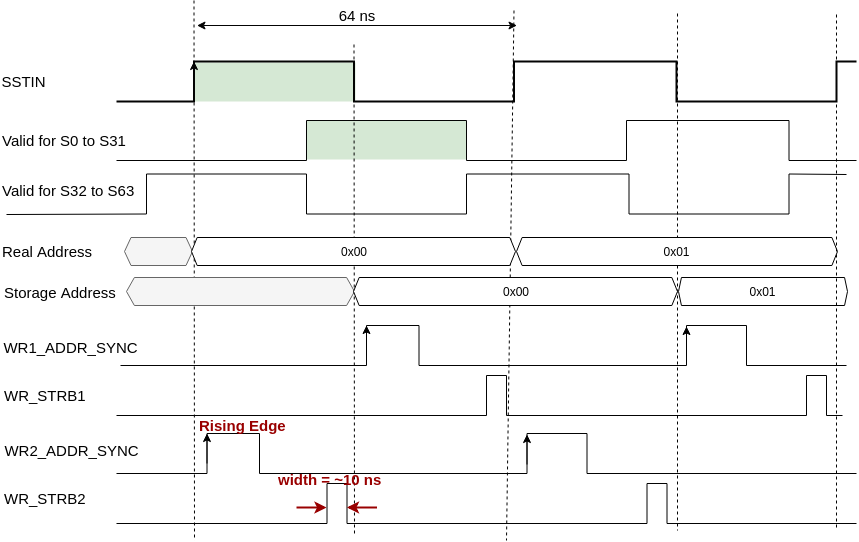
\includegraphics[width=0.8\textwidth]{figures/SSTIN_signals.png}\\
  \caption{\label{fig:sstinsignals} Timing principle for write address and write strobe signals}
\end{figure}

\subsubsection*{Pinout(s)}
WR\_RS\_S are the lower bits and WR\_CS\_S are the upper bits of the storage address.
\begin{table}[H]
\centering
\begin{tabu}{   | c | p{0.15\linewidth} | p{0.2\linewidth} | p{0.4\linewidth} |}
\hline
\HEADTABLE
Pin\# & Pin Name & Pin Type & Description\\
\hline
46	& WR\_RS\_S0	& Digital Input & WR Row Select Addr. 0	 \\
47	& WR\_RS\_S1	& Digital Input & WR Row Select Addr. 1	 \\
48	& WR\_CS\_S0	& Digital Input & WR Column Select Addr. 0	 \\
49	& WR\_CS\_S1	& Digital Input & WR Column Select Addr. 1	 \\
50	& WR\_CS\_S2	& Digital Input & WR Column Select Addr. 2	 \\
51	& WR\_CS\_S3	& Digital Input & WR Column Select Addr. 3	 \\
54	& WR\_CS\_S4	& Digital Input& WR Column Select Addr. 4	\\
55	& WR\_CS\_S5	& Digital Input& WR Column Select Addr. 5	\\
\hline
\end{tabu}
\caption{\label{tab:storeaddr} Storage address interface Pins}
\end{table}

\subsubsection*{Requirement(s)}
\begin{table}[H]
\centering
\begin{tabu}{   | p{0.1\linewidth} | p{0.8\linewidth} |}
\hline
\HEADTABLE
Req\# & Description\\
\hline
1	& WR\_RS\_S(1-0) and WR\_CS\_S(5-0) shall be updated on the falling edge. \\
\hline
\end{tabu}
\caption{\label{tab:reqregwrite} Requirement for the register write interface ({\tiny Update : 28th of January 2019})}
\end{table}


\subsubsection*{Interface sequence}

\begin{figure}[H]
\centering
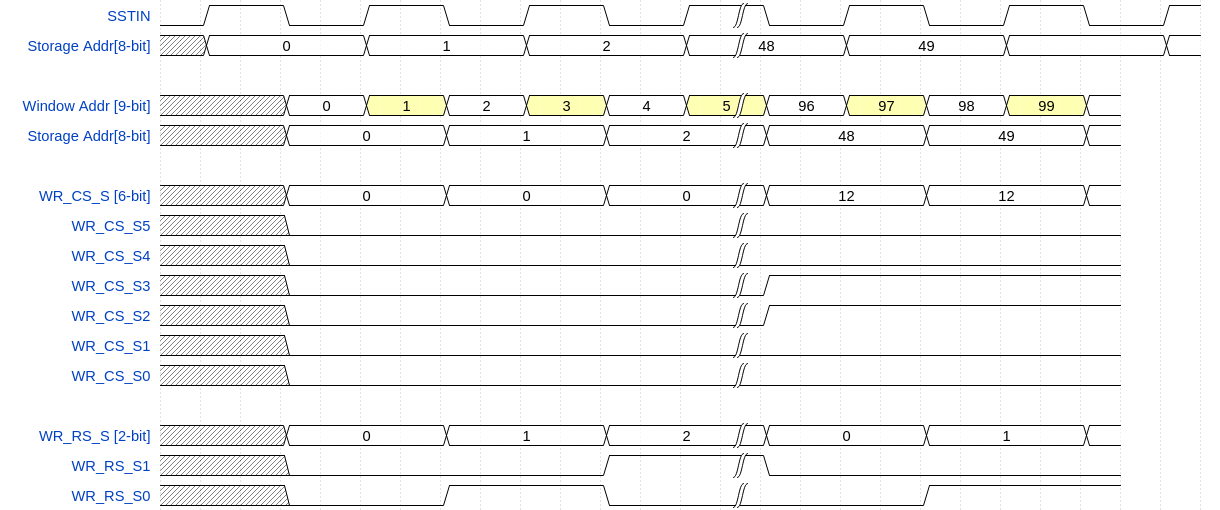
\includegraphics[width=1\textwidth]{figures/wavedrom/storageaddr_correct.png}\\
\caption{\label{fig:storageaddr}Storage address update sequence ({\tiny Update : 28th of January 2019})}
\end{figure}


%%%%%%%%%%%%%%%%%%%%%%%%%%%%%%%%%%%%%%%%%%%%%%%%%%%%%%%%%%%%%%%%
\subsection{Window Readout}
As mentioned the storage address is a 8-Bit wide address. The readout is a 9-Bit address, the extra bit enables the selection between the 1st or 2nd window sampled. In the TARGET world, we speak of EVEN or ODD window, the 1st window being the EVEN and respectively the 2nd the ODD window.

\begin{figure}[H]
\centering
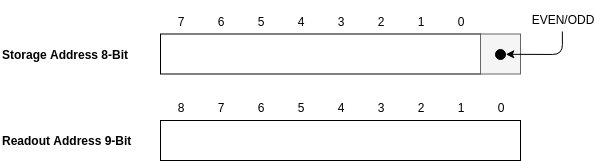
\includegraphics[width=0.7\textwidth]{figures/StorageReadoutAddr.png}\\
\caption{\label{fig:StorageReadoutAddr}Storage VS Readout address}
\end{figure}

\noindent
From previous TARGET designs, the readout address is swapped and the extra bit is placed in different places. This should not be the case for TARGETC.

\subsubsection*{Pinout(s)}
\begin{table}[H]
\centering
\begin{tabu}{   | c | p{0.15\linewidth} | p{0.2\linewidth} | p{0.4\linewidth} |}
\hline
\HEADTABLE
Pin\# & Pin Name & Pin Type & Description\\
\hline
61	& RDAD\_clk	& Digital Input & Read Address Set SCLK	 \\
62	& RDAD\_sin	& Digital Input& Read Address Set Serial Input	\\
63	& RDAD\_dir	& Digital Input& Read Address Set DIR	 \\
\hline
\end{tabu}
\caption{\label{tab:readoutpins} Read address interface Pins}
\end{table}

\subsubsection*{Requirement(s)}
\begin{table}[H]
\centering
\begin{tabu}{   | p{0.1\linewidth} | p{0.8\linewidth} |}
\hline
\HEADTABLE
Req\# & Description\\
\hline
1	& TARGETC samples on the rising edge of RDAD\_CLK. Data shall be shifted during the LOW period of the clock on SIN.\\
2 & MSB is shifted out first on RDAD\_SIN\\
\hline
\end{tabu}
\caption{\label{tab:readoutreq} Requirement for the readout interface}
\end{table}

\subsubsection*{Interface sequence}
\begin{figure}[H]
\centering
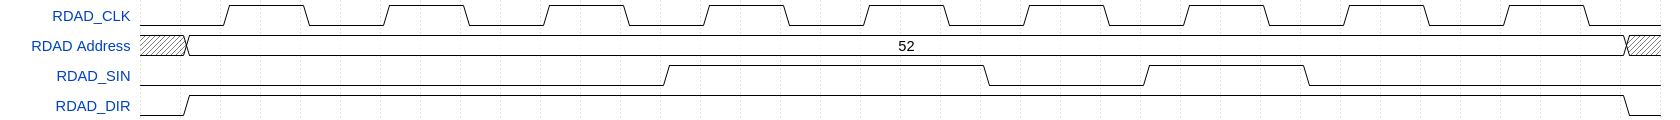
\includegraphics[width=1\textwidth]{figures/wavedrom/readoutseq.png}\\
\caption{\label{fig:readoutseq}Example of Readout Address sequence for window $52_{10}$}
\end{figure}

%%%%%%%%%%%%%%%%%%%%%%%%%%%%%%%%%%%%%%%%%%%%%%%%%%%%%%%%%%%%%%%%
\newpage
\subsection{Wilkinson Digitization}
The read module inside the ASIC decodes the address entered on the readout interface and the corresponding internal switches are powered on, connecting the window's cells comparator outputs to the latch inputs of the sample registers (Output shift register). The Wilkinson counter is reset using the signal GCC\_Reset (11-Bit Gray Code Counter). The ramp signal (eRamp) is enabled, which enables the charge of the Wilkinson capacitor. It is important to synchronize eRamp signal with the release of GCC\_reset signal, because the counter is incrementing on every rising edge of the Wilkinson clock. Once the comparator stored value is equal to the capacitor's value, the comparator's output switches from LOW to HIGH, this has the effect of latching the counter's value in the sample register. This latched value corresponds to the gray coded digital value of the stored sample. After the digitization is completed the eRamp signal must be kept HIGH during all the sample readout. Finally the Wilkinson capacitor should have enough time to discharge completely.

\begin{figure}[H]
\centering
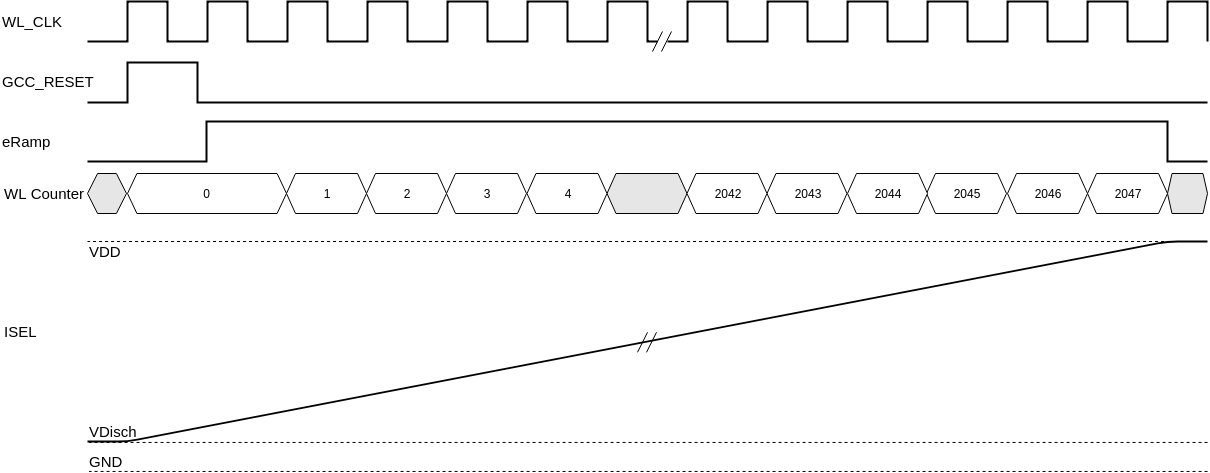
\includegraphics[width=1\textwidth]{figures/ISELWL.png}\\
\caption{\label{fig:iselclock}Wilkinson conversion signals for full range (VDD=2047)}
\end{figure}

\subsubsection*{Pinout(s)}
\begin{table}[H]
\centering
\begin{tabu}{   | c | p{0.15\linewidth} | p{0.2\linewidth} | p{0.4\linewidth} |}
\hline
\HEADTABLE
Pin\# & Pin Name & Pin Type & Description\\
\hline
56	& GCC\_Reset & Digital Input & Gray Code Counter Reset	\\
57	& WL\_CLK\_n & LVDS Input & Wilkinson Clock LVDS	 \\
58	& WL\_CLK\_p & LVDS Input & Wilkinson Clock LVDS	 \\
108	& eRamp		& Digital Input & Wilkinson Ramp control	\\
110	& Vdischarge & Analog Output	& Wilkinson Ramp Start voltage	\\
111	& RampMon	& Analog Output	& Buffered copy of Wilk Ramp	\\
112	& ISEL		& Analog Output	& Monitor for Wilk Ramp I (V out)	\\
113	& VrampRef	& Analog Output	& Charging node	\\
\hline
\end{tabu}
\caption{\label{tab:storeaddr} Storage address interface Pins}
\end{table}


\subsubsection*{Requirement(s)}
\begin{table}[H]
\centering
\begin{tabu}{   | p{0.1\linewidth} | p{0.8\linewidth} |}
\hline
\HEADTABLE
Req\# & Description\\
\hline
1	& The Wilkinson frequency must correspond with the charge of the capacitor defined by the DAC register ISEL.\\
2 & The counter must be reset before starting a new conversion.\\
3 & The eRamp signal is held HIGH during all sample readout.\\
\hline
\end{tabu}
\caption{\label{tab:wilkinsonReg} Requirement for the wilkinson interface}
\end{table}


\subsubsection*{Interface sequence}
\begin{figure}[H]
\centering
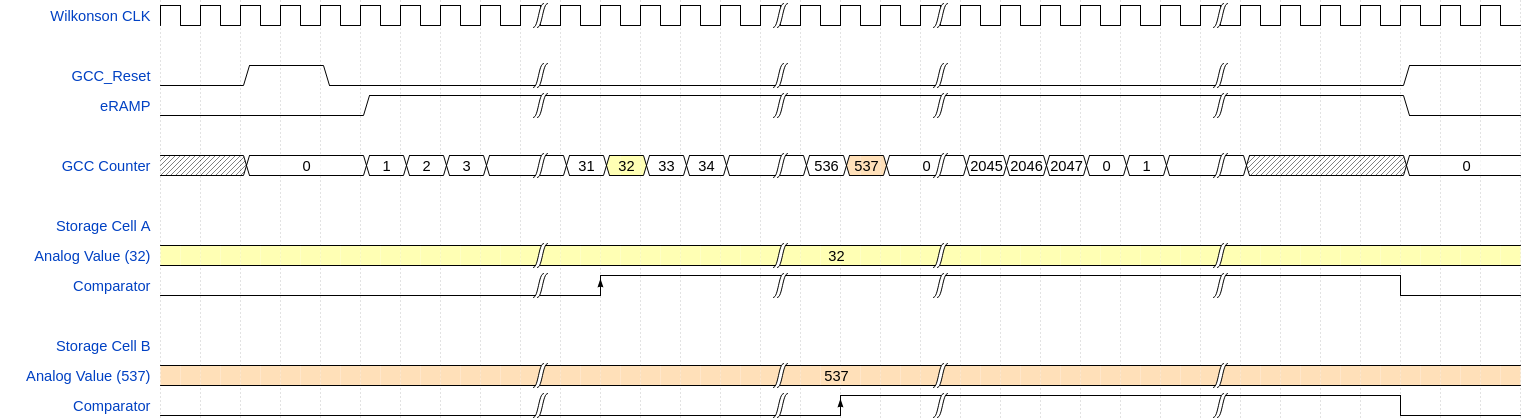
\includegraphics[width=1\textwidth]{figures/wavedrom/wilkinsonseq.png}\\
\caption{\label{fig:wilkinsonseq} Wilkinson sequence for the digitization of a selected window}
\end{figure}

%%%%%%%%%%%%%%%%%%%%%%%%%%%%%%%%%%%%%%%%%%%%%%%%%%%%%%%%%%%%%%%%
\subsection{Sample Readout}
The sample readout is an internal counter that can be incremented on the rising edge of SS\_Incr or reset using eSS\_Reset (Active HIGH). Once the 32 samples from all channels have been read, the counter goes back to sample 0 by applying a pulse on SS\_Incr. The falling edge of SS\_Incr charges the values into the registers. This is why the pulse width is important, because of the disposition of the registers in the ASIC, some lines take longer than others to arrive. The pulse should be long enough for the data to be stable before latching it into the output registers.

\subsubsection*{Pinout(s)}
\begin{table}[H]
\centering
\begin{tabu}{   | c | p{0.15\linewidth} | p{0.2\linewidth} | p{0.4\linewidth} |}
\hline
\HEADTABLE
Pin\# & Pin Name & Pin Type & Description\\
\hline
43	& HSclkN	& LVDS Input & Data Shift-out Clock	\\
44	& HSclkP	& LVDS Input & LVDS	\\
66	& SmplSl\_Any & Digital Input & Select between TPG or sample value\\
79	& SS\_Incr	& Digital Input & Sample Select increment	\\
80	& DOE		& Digital Input & Data Output Enable\\
69	& DO\_16	& Digital Output & Serial Data Out Ch. 16	\\
70	& DO\_15	& Digital Output & Serial Data Out Ch. 15	\\
71	& DO\_14	& Digital Output & Serial Data Out Ch. 14	\\
72	& DO\_13	& Digital Output & Serial Data Out Ch. 13	\\
73	& DO\_12	& Digital Output & Serial Data Out Ch. 12	\\
74	& DO\_11	& Digital Output & Serial Data Out Ch. 11	\\
75	& DO\_10	& Digital Output & Serial Data Out Ch. 10	\\
76	& DO\_9		& Digital Output & Serial Data Out Ch. 9	\\
84	& DO\_8		& Digital Output & Serial Data Out Ch. 8	\\
85	& DO\_7		& Digital Output & Serial Data Out Ch. 7	\\
86	& DO\_6		& Digital Output & Serial Data Out Ch. 6	\\
87	& DO\_5		& Digital Output & Serial Data Out Ch. 5	\\
88	& DO\_4		& Digital Output & Serial Data Out Ch. 4	\\
89	& DO\_3		& Digital Output & Serial Data Out Ch. 3	\\
90	& DO\_2		& Digital Output & Serial Data Out Ch. 2	\\
91	& DO\_1		& Digital Output & Serial Data Out Ch. 1	\\
95	& eSS\_Reset	& Digital input & Sample Select reset	\\
\hline
\end{tabu}
\caption{\label{tab:sspins} Sample Readout interface Pins}
\end{table}



\subsubsection*{Requirement(s)}
\begin{table}[H]
\centering
\begin{tabu}{   | p{0.1\linewidth} | p{0.8\linewidth} |}
\hline
\HEADTABLE
Req\# & Description\\
\hline
1	& SS\_Incr pulse shall be wide enough (latency in ASIC).\\
\hline
\end{tabu}
\caption{\label{tab:ssreq} Requirement for the sample select interface}
\end{table}


\subsubsection*{Interface sequence}
\noindent
The interface sequence is very particular for the first sample. The SS\_Reset is brought LOW and after the SS\_INCR is brought HIGH. Internally this effect will load the register of sample 0 on the bus. After a stabilization time, SS\_Reset is disabled and then SS\_INCR is set LOW. The data of the register will be latched into the output shift register.
\begin{figure}[H]
\centering
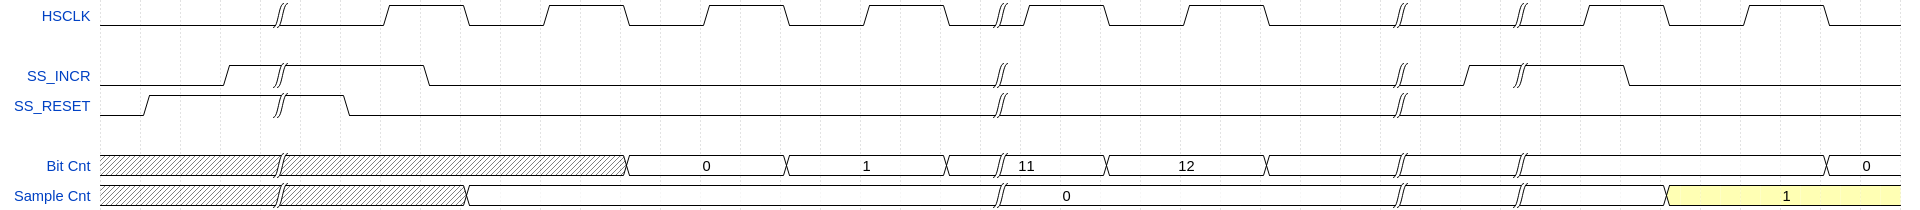
\includegraphics[width=1\textwidth]{figures/wavedrom/ssseq.png}\\
\caption{\label{fig:ssseq} Sample select readout sequence}
\end{figure}
